\documentclass[11pt]{article}

\usepackage{fullpage}
\usepackage{amsmath, amssymb, bm, cite, epsfig, psfrag}
\usepackage{graphicx}
\usepackage{float}
\usepackage{amsthm}
\usepackage{amsfonts}
\usepackage{listings}
\usepackage{cite}
\usepackage{hyperref}
\usepackage{tikz}
\usepackage{enumerate}
\usepackage[outercaption]{sidecap}
\usetikzlibrary{shapes,arrows}
%\usetikzlibrary{dsp,chains}

%\restylefloat{figure}
%\theoremstyle{plain}      \newtheorem{theorem}{Theorem}
%\theoremstyle{definition} \newtheorem{definition}{Definition}

\def\del{\partial}
\def\ds{\displaystyle}
\def\ts{\textstyle}
\def\beq{\begin{equation}}
\def\eeq{\end{equation}}
\def\beqa{\begin{eqnarray}}
\def\eeqa{\end{eqnarray}}
\def\beqan{\begin{eqnarray*}}
\def\eeqan{\end{eqnarray*}}
\def\nn{\nonumber}
\def\binomial{\mathop{\mathrm{binomial}}}
\def\half{{\ts\frac{1}{2}}}
\def\Half{{\frac{1}{2}}}
\def\N{{\mathbb{N}}}
\def\Z{{\mathbb{Z}}}
\def\Q{{\mathbb{Q}}}
\def\R{{\mathbb{R}}}
\def\C{{\mathbb{C}}}
\def\argmin{\mathop{\mathrm{arg\,min}}}
\def\argmax{\mathop{\mathrm{arg\,max}}}
%\def\span{\mathop{\mathrm{span}}}
\def\diag{\mathop{\mathrm{diag}}}
\def\x{\times}
\def\limn{\lim_{n \rightarrow \infty}}
\def\liminfn{\liminf_{n \rightarrow \infty}}
\def\limsupn{\limsup_{n \rightarrow \infty}}
\def\GV{Guo and Verd{\'u}}
\def\MID{\,|\,}
\def\MIDD{\,;\,}

\newtheorem{proposition}{Proposition}
\newtheorem{definition}{Definition}
\newtheorem{theorem}{Theorem}
\newtheorem{lemma}{Lemma}
\newtheorem{corollary}{Corollary}
\newtheorem{assumption}{Assumption}
\newtheorem{claim}{Claim}
\def\qed{\mbox{} \hfill $\Box$}
\setlength{\unitlength}{1mm}

\def\bhat{\widehat{b}}
\def\ehat{\widehat{e}}
\def\phat{\widehat{p}}
\def\qhat{\widehat{q}}
\def\rhat{\widehat{r}}
\def\shat{\widehat{s}}
\def\uhat{\widehat{u}}
\def\ubar{\overline{u}}
\def\vhat{\widehat{v}}
\def\xhat{\widehat{x}}
\def\xbar{\overline{x}}
\def\zhat{\widehat{z}}
\def\zbar{\overline{z}}
\def\la{\leftarrow}
\def\ra{\rightarrow}
\def\MSE{\mbox{\small \sffamily MSE}}
\def\SNR{\mbox{\small \sffamily SNR}}
\def\SINR{\mbox{\small \sffamily SINR}}
\def\arr{\rightarrow}
\def\Exp{\mathbb{E}}
\def\var{\mbox{var}}
\def\Tr{\mbox{Tr}}
\def\tm1{t\! - \! 1}
\def\tp1{t\! + \! 1}

\def\Xset{{\cal X}}

\newcommand{\one}{\mathbf{1}}
\newcommand{\abf}{\mathbf{a}}
\newcommand{\bbf}{\mathbf{b}}
\newcommand{\dbf}{\mathbf{d}}
\newcommand{\ebf}{\mathbf{e}}
\newcommand{\gbf}{\mathbf{g}}
\newcommand{\hbf}{\mathbf{h}}
\newcommand{\pbf}{\mathbf{p}}
\newcommand{\pbfhat}{\widehat{\mathbf{p}}}
\newcommand{\qbf}{\mathbf{q}}
\newcommand{\qbfhat}{\widehat{\mathbf{q}}}
\newcommand{\rbf}{\mathbf{r}}
\newcommand{\rbfhat}{\widehat{\mathbf{r}}}
\newcommand{\sbf}{\mathbf{s}}
\newcommand{\sbfhat}{\widehat{\mathbf{s}}}
\newcommand{\ubf}{\mathbf{u}}
\newcommand{\ubfhat}{\widehat{\mathbf{u}}}
\newcommand{\utildebf}{\tilde{\mathbf{u}}}
\newcommand{\vbf}{\mathbf{v}}
\newcommand{\vbfhat}{\widehat{\mathbf{v}}}
\newcommand{\wbf}{\mathbf{w}}
\newcommand{\wbfhat}{\widehat{\mathbf{w}}}
\newcommand{\xbf}{\mathbf{x}}
\newcommand{\xbfhat}{\widehat{\mathbf{x}}}
\newcommand{\xbfbar}{\overline{\mathbf{x}}}
\newcommand{\ybf}{\mathbf{y}}
\newcommand{\zbf}{\mathbf{z}}
\newcommand{\zbfbar}{\overline{\mathbf{z}}}
\newcommand{\zbfhat}{\widehat{\mathbf{z}}}
\newcommand{\Ahat}{\widehat{A}}
\newcommand{\Abf}{\mathbf{A}}
\newcommand{\Bbf}{\mathbf{B}}
\newcommand{\Cbf}{\mathbf{C}}
\newcommand{\Bbfhat}{\widehat{\mathbf{B}}}
\newcommand{\Dbf}{\mathbf{D}}
\newcommand{\Gbf}{\mathbf{G}}
\newcommand{\Hbf}{\mathbf{H}}
\newcommand{\Kbf}{\mathbf{K}}
\newcommand{\Pbf}{\mathbf{P}}
\newcommand{\Phat}{\widehat{P}}
\newcommand{\Qbf}{\mathbf{Q}}
\newcommand{\Rbf}{\mathbf{R}}
\newcommand{\Rhat}{\widehat{R}}
\newcommand{\Sbf}{\mathbf{S}}
\newcommand{\Ubf}{\mathbf{U}}
\newcommand{\Vbf}{\mathbf{V}}
\newcommand{\Wbf}{\mathbf{W}}
\newcommand{\Xhat}{\widehat{X}}
\newcommand{\Xbf}{\mathbf{X}}
\newcommand{\Ybf}{\mathbf{Y}}
\newcommand{\Zbf}{\mathbf{Z}}
\newcommand{\Zhat}{\widehat{Z}}
\newcommand{\Zbfhat}{\widehat{\mathbf{Z}}}
\def\alphabf{{\boldsymbol \alpha}}
\def\betabf{{\boldsymbol \beta}}
\def\mubf{{\boldsymbol \mu}}
\def\lambdabf{{\boldsymbol \lambda}}
\def\etabf{{\boldsymbol \eta}}
\def\xibf{{\boldsymbol \xi}}
\def\taubf{{\boldsymbol \tau}}
\def\sigmahat{{\widehat{\sigma}}}
\def\thetabf{{\bm{\theta}}}
\def\thetabfhat{{\widehat{\bm{\theta}}}}
\def\thetahat{{\widehat{\theta}}}
\def\mubar{\overline{\mu}}
\def\muavg{\mu}
\def\sigbf{\bm{\sigma}}
\def\etal{\emph{et al.}}
\def\Ggothic{\mathfrak{G}}
\def\Pset{{\mathcal P}}
\newcommand{\bigCond}[2]{\bigl({#1} \!\bigm\vert\! {#2} \bigr)}
\newcommand{\BigCond}[2]{\Bigl({#1} \!\Bigm\vert\! {#2} \Bigr)}

\def\Rect{\mathop{Rect}}
\def\sinc{\mathop{sinc}}
\def\Real{\mathrm{Re}}
\def\Imag{\mathrm{Im}}



\begin{document}

\title{Problems:  Symbol Mapping and TX Filtering}
\author{Prof.\ Sundeep Rangan}
\date{}

\maketitle

\begin{enumerate}

\item \emph{Symbol mapping.}  Suppose a sequence of bits $b[k]$ are mapped to a
16-QAM constellation shown in Fig.~\ref{fig:QAM16} where the constellation
points are $s[n] = s_I[n] + js_Q[n]$ with $s_c[n], s_s[n] \in \{ -3,-1,1,3\}$.
Then, the symbols are modulated to produce a complex baseband signal $u(t)$,
\[
    u(t) = \sum_{n=-\infty}^\infty b[n]p(t-nT),
\]
for some pulse shape $p(t)$.

\begin{SCfigure}[50][h]
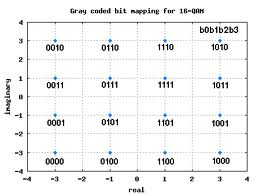
\includegraphics[width=8cm]{QAM16.jpg}
\caption{16-QAM constellation with gray coded bit labels.   } \label{fig:QAM16}
\end{SCfigure}

\begin{enumerate}[(a)]
\item For an information rate of 80 Mbps, what should the value of $T$ be?  State your units.

\item Suppose the sequence of bits is $\mathbf{b}
= (0,1,1,0, 1,1,0,1, 0,1,0,0)$ starting at $b[0]$.
Assume the bits are read from left to right so that
\[
    (b[4n],b[4n+1],b[4n+2],b[4n+3]) \mapsto (b_0,b_1,b_2,b_3)
\]
where $(b_0,b_1,b_2,b_3)$ are shown as the labels in the figure.
What are the sequence of symbols $s[n]$ resulting from the bits $b[k]$?

\item Suppose that the pulse shape is
\[
    p(t) = A\max\left\{0, 1-|t/T|\right\}
\]
Draw $p(t)$.

\item Draw the real and imaginary parts of $u(t)$ for the above symbols
and pulse shape.
\end{enumerate}


\item \emph{PSD.}  Suppose we use linear modulation,
\[
    u(t) = \sum_n s[n]p(t-nT),
\]
where
\begin{itemize}
\item The symbol rate is $\frac{1}{T}=20$ Msym/s;
\item The pulse shape is
$p(t)=\sqrt{P_0}e^{-t/T}I_{[0,\infty)}(t)$, where $P_0 = 10$ mW.
\item   The PSD of the symbols $s[n]$
is $S_s(\Omega) = C\Rect(\Omega/\Omega_0)$ where $\Omega_0 = 1.6\pi$.
\end{itemize}

\begin{enumerate}[(a)]

\item If $\Exp|s[n]|^2 = 1$, find $C$.

\item Draw the PSD, $S_u(f)$ of $u(t)$.
Make sure you label your axes.

\item What is the power in the main lobe (in dBm).

\item What is the power in the first sidelobe (in dBm)?  Only compute the power
of the sidelobe in the right frequencies.
\end{enumerate}

\item \label{prob:up_filter}
\emph{Upsampling filter design.}  
A sequence of symbols $s[n]$ have a symbol rate of $1/T=30$ MHz and PSD, $S(\Omega)$ shown in 
the top panel of Fig.~\ref{fig:up_filter}.  Assume the signal of interest
is contained in $|\Omega| < 0.8\pi$.  
 
\begin{enumerate}
\item The signal is up-sampled by a factor of $M=2$ to create a new signal $v[k]$.
Assume the upsampling uses zero insertion.
What is the sample rate of $v[k]$?
Draw the PSD, $S_v(\Omega)$.  Make sure you label the axes.

\item The upsampled signal $v[k]$ is then filtered to produce $w[k] = h[k]*v[k]$ 
where the power gain of $|H(f)|^2$ is shown in the middle panel of Fig.~\ref{fig:up_filter}.
Assume $\Omega_0=0.4\pi$ and $\Omega_1=0.6\pi$.
Draw the PSD $S_w(\Omega)$.

\item The filtered signal $w[k]$ is then linearly modulated to produce 
$u(t) = \sum_k w[k]p(t-kT/2)$ where the power gain of the pulse shape is shown in the bottom
panel of Fig.~\ref{prob:up_filter}.  Select the parameters of the pulse shape filters,
$f_0,f_1,G_0,G_1$ such that:
\begin{itemize}
\item The PSD $S_u(f)$ is flat in the region of the signal of interest 
(i.e.\ $|f|\leq 12$ MHz).
\item The PSD $S_u(f)$ is at least 40 dB below the peak PSD for all $|f|>18$ MHz.
\item The total power in the signal of interest is 15 dBm.
\item The filter has the widest transition bandwidth $(f_1-f_0)$ and minimum
stopband rejection ($G_0-G_1$) as possible.
\end{itemize}
Draw the resulting PSD $S_u(f)$.
\end{enumerate}

\begin{figure}
\center
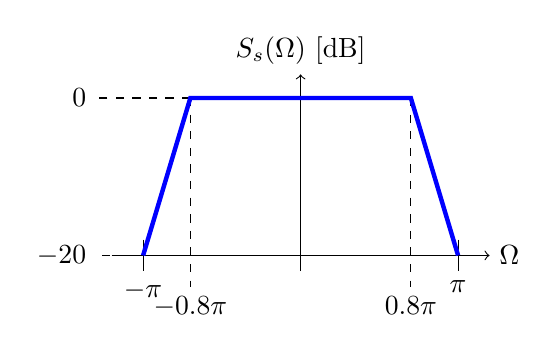
\begin{tikzpicture}[xscale=2,yscale=1]
    \pgfmathsetmacro{\fa}{0.7}
    \pgfmathsetmacro{\fm}{1}
    \pgfmathsetmacro{\A}{2}
    \pgfmathsetmacro{\tic}{0.2}    
    \pgfmathsetmacro{\ticb}{0.4}
    % Draw the axes
    \draw [->] (-1.2,0) -- (1.2,0) node [right] {$\Omega$};
    \draw [->] (0,-\tic) -- (0,2.3) node [above] {$S_s(\Omega)$ [dB]};
    \draw [-] (\fm,\tic) -- (\fm,-\tic) node [below] {$\pi$};
    \draw [-] (-\fm,\tic) -- (-\fm,-\tic) node [below] {$-\pi$};
    \draw [-,dashed] (-\fa,\A) -- (-\fa,-\ticb) node [below] {$-0.8\pi$};
    \draw [-,dashed] (\fa,\A) -- (\fa,-\ticb) node [below] {$0.8\pi$};
    \draw [-,dashed] (-\fa,\A) -- (-1.3,\A) node [left] {$0$};
    \draw [-,dashed] (-\fm,0) -- (-1.3,0) node [left] {$-20$};

    % Draw Real S_u(\Omega)
    \draw [ultra thick,blue,-] (-\fm,0) -- (-\fa,\A) -- (\fa,\A) -- (\fm,0);

\end{tikzpicture}

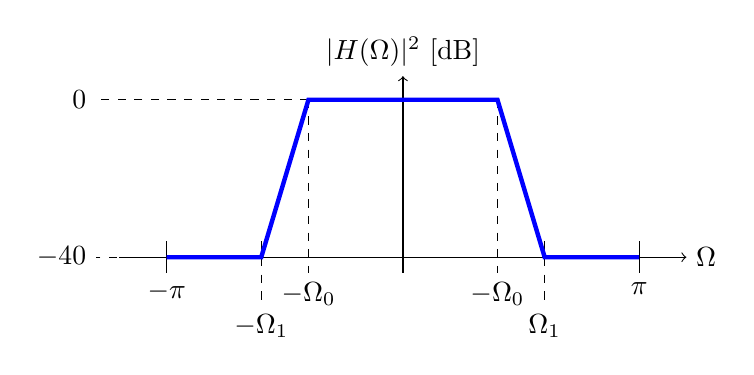
\begin{tikzpicture}[xscale=3,yscale=1]
    \pgfmathsetmacro{\fa}{0.4}
    \pgfmathsetmacro{\fb}{0.6}
    \pgfmathsetmacro{\fm}{1}
    \pgfmathsetmacro{\A}{2}
    \pgfmathsetmacro{\tic}{0.2}
    \pgfmathsetmacro{\ticb}{0.6}
    % Draw the axes
    \draw [->] (-1.2,0) -- (1.2,0) node [right] {$\Omega$};
    \draw [->] (0,-\tic) -- (0,2.3) node [above] {$|H(\Omega)|^2$ [dB]};
    \draw [-] (\fm,\tic) -- (\fm,-\tic) node [below] {$\pi$};
    \draw [-] (-\fm,\tic) -- (-\fm,-\tic) node [below] {$-\pi$};
    \draw [-,dashed] (-\fa,\A) -- (-\fa,-\tic) node [below] {$-\Omega_0$};
    \draw [-,dashed] (\fa,\A) -- (\fa,-\tic) node [below] {$-\Omega_0$};
    \draw [-,dashed] (-\fb,\tic) -- (-\fb,-\ticb) node [below] {$-\Omega_1$};
    \draw [-,dashed] (\fb,\tic) -- (\fb,-\ticb) node [below] {$\Omega_1$};
    
    
    \draw [-,dashed] (-\fa,\A) -- (-1.3,\A) node [left] {$0$};
    \draw [-,dashed] (-\fm,0) -- (-1.3,0) node [left] {$-40$};
    
    % Draw Real S_u(\Omega)
    \draw [ultra thick,blue,-] (-\fm,0) -- (-\fb,0) -- 
        (-\fa,\A) -- (\fa,\A) -- (\fb,0) -- (\fm,0);

\end{tikzpicture}

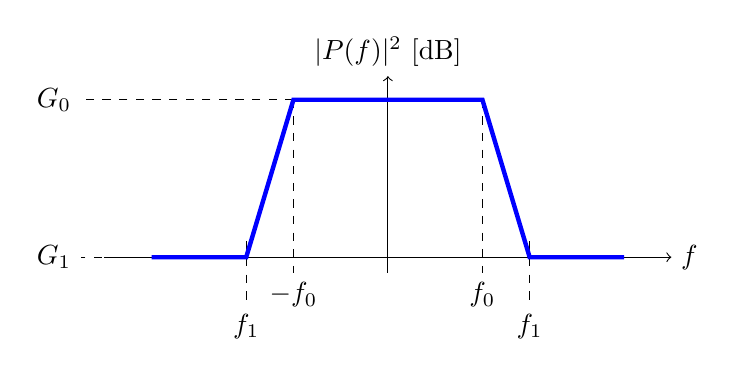
\begin{tikzpicture}[xscale=3,yscale=1]
    \pgfmathsetmacro{\fa}{0.4}
    \pgfmathsetmacro{\fb}{0.6}
    \pgfmathsetmacro{\fm}{1}
    \pgfmathsetmacro{\A}{2}
    \pgfmathsetmacro{\tic}{0.2}
    \pgfmathsetmacro{\ticb}{0.6}
    % Draw the axes
    \draw [->] (-1.2,0) -- (1.2,0) node [right] {$f$};
    \draw [->] (0,-\tic) -- (0,2.3) node [above] {$|P(f)|^2$ [dB]};
    \draw [-,dashed] (-\fa,\A) -- (-\fa,-\tic) node [below] {$-f_0$};
    \draw [-,dashed] (\fa,\A) -- (\fa,-\tic) node [below] {$f_0$};
    \draw [-,dashed] (-\fb,\tic) -- (-\fb,-\ticb) node [below] {$f_1$};
    \draw [-,dashed] (\fb,\tic) -- (\fb,-\ticb) node [below] {$f_1$};
    
    \draw [-,dashed] (-\fa,\A) -- (-1.3,\A) node [left] {$G_0$};
    \draw [-,dashed] (-\fm,0) -- (-1.3,0) node [left] {$G_1$};

    % Draw Real S_u(\Omega)
    \draw [ultra thick,blue,-] (-\fm,0) -- (-\fb,0) --
        (-\fa,\A) -- (\fa,\A) -- (\fb,0) -- (\fm,0);

\end{tikzpicture}
\caption{PSDs and filter responses for Problem~\ref{prob:up_filter}.
Note values are in dB scale.} \label{fig:up_filter}
\end{figure}


\end{enumerate}

\end{document}
